\documentclass[12pt, letterpaper]{article}
\usepackage[margin=1in]{geometry}
\usepackage{mathptmx}
\usepackage{amsmath}
\usepackage{graphicx}
\usepackage{booktabs}
\usepackage{multirow}
\usepackage[font={small,it}, justification=centering, labelfont=bf]{caption}
\usepackage{float}
\usepackage[skip=4pt]{parskip}
\usepackage{hyperref}
\hypersetup{colorlinks=true, linkcolor=blue, urlcolor=blue}
\usepackage{tikz}
\usetikzlibrary{automata, positioning, arrows.meta}
\usepackage{titlesec}
\titlespacing*{\section}{0pt}{8pt}{4pt}
\titlespacing*{\subsection}{0pt}{6pt}{2pt}
\usepackage{listings}
\usepackage{xcolor}

% Roman numeral section counter
\renewcommand{\thesection}{\Roman{section}}
\titleformat{\section}{\normalfont\bfseries\large}{\thesection.}{0.5em}{}

% Simple arabic numbering for subsections
\renewcommand{\thesubsection}{\arabic{subsection}}
\titleformat{\subsection}{\normalfont\bfseries}{\thesubsection.}{0.5em}{}

\lstdefinestyle{verilog}{
  language=Verilog,
  basicstyle=\ttfamily\footnotesize,
  keywordstyle=\color{blue}\bfseries,
  commentstyle=\color{gray}\itshape,
  stringstyle=\color{orange},
  numbers=left,
  numberstyle=\tiny\color{gray},
  stepnumber=1,
  frame=single,
  breaklines=true,
  tabsize=2,
  showstringspaces=false,
}

\begin{document}

\begin{center}
  {\Large \textbf{Report for CDA 3201L Lab \#7}}\\[10pt]
  {\large \textbf{Sequential Circuits -- Gray Code Counter}}\\[20pt]
  \begin{tabular}{ll}
    \textbf{Name:} Tuan Khang Phan & \textbf{UID:} U30382645 \\[4pt]
    \textbf{Name:} Huu Phat Nguyen & \textbf{UID:} U46082380 \\
  \end{tabular}
\end{center}

% ─────────────────────────────────────────────
\section{Introduction}

The purpose of this lab is to deepen our understanding of sequential circuit design by
designing and implementing a 3-bit Gray code up counter using D flip-flops (DFFs).
Unlike a standard binary counter, a Gray code counter changes only one bit per clock
cycle, making it useful for minimizing switching errors in digital systems.  We used the
74LS74 dual-DFF IC as our memory element, minimized the combinational next-state logic
using Karnaugh maps, and implemented the resulting NAND-NAND two-level logic on a
breadboard.  The circuit output was displayed using three LEDs and later extended to
include a 74LS47N BCD-to-7-segment decoder/driver and a 7-segment display.

% ─────────────────────────────────────────────
\section{Methods and Materials}

We used the following components and equipment:

\begin{itemize}
  \item Two SN74LS109AN dual positive edge-triggered JK flip-flop ICs (configured as
        DFFs by connecting $J = D$ and $\overline{K} = D$; provides both $Q$ and
        $\overline{Q}$ outputs; asynchronous active-low CLR used for reset)
  \item One SN74LS08N quad 2-input AND gate IC
  \item One SN74LS86AN quad 2-input XOR gate IC
  \item One SN74LS04N hex inverter IC
  \item Three LEDs and current-limiting resistors (for original circuit)
  \item SN74LS47N BCD-to-7-segment decoder/driver and common-anode 7-segment display
        (for modified circuit)
  \item One push button and pull-up resistor (for active-low reset)
  \item Breadboard and jumper wires
  \item 5\,V DC power supply
  \item Function generator (1\,Hz square wave, CMOS output, for clock)
\end{itemize}

We first derived the 3-bit Gray code next-state table for the sequence
$000 \to 001 \to 011 \to 010 \to 110 \to 111 \to 101 \to 100 \to 000$.
Since the DFF characteristic equation is $Q^* = D$, the D inputs equal the desired
next states directly.  We filled in three Karnaugh maps to obtain minimized SOP
expressions for $D_2$, $D_1$, and $D_0$.  The SN74LS109AN is a JK flip-flop with a
$\overline{K}$ input; connecting $J = D$ and $\overline{K} = D$ configures it as a DFF.
Its $\overline{Q}$ outputs supply all complemented state signals needed by the
combinational logic.  The simplified equations were implemented using AND gates
(SN74LS08N) and XOR gates (SN74LS86AN), with the SN74LS04N providing the single
inversion required for $D_0$.  After confirming the design with the TA, we wired the
circuit on the breadboard, connected a 1\,Hz clock from the function generator, and
verified correct operation using the LED outputs.  In the extension, we replaced the
LEDs with the SN74LS47N and 7-segment display.

% ─────────────────────────────────────────────
\section{Results}

\subsection{Verilog Behavioral Model, Testbench, and Waveform}

The following Verilog module describes the 3-bit Gray code counter behaviorally using a
\texttt{case} statement that encodes the Gray code sequence directly:

\begin{lstlisting}[style=verilog, caption={Behavioral Verilog model for the 3-bit Gray code counter.}]
module gray_counter (
    input        clk,
    input        reset,
    output reg [2:0] Q
);
    always @(posedge clk or posedge reset) begin
        if (reset)
            Q <= 3'b000;
        else begin
            case (Q)
                3'b000: Q <= 3'b001;
                3'b001: Q <= 3'b011;
                3'b011: Q <= 3'b010;
                3'b010: Q <= 3'b110;
                3'b110: Q <= 3'b111;
                3'b111: Q <= 3'b101;
                3'b101: Q <= 3'b100;
                3'b100: Q <= 3'b000;
                default: Q <= 3'b000;
            endcase
        end
    end
endmodule
\end{lstlisting}

\begin{lstlisting}[style=verilog, caption={Testbench for the 3-bit Gray code counter.}]
module gray_counter_tb;
    reg        clk, reset;
    wire [2:0] Q;

    gray_counter uut (
        .clk   (clk),
        .reset (reset),
        .Q     (Q)
    );

    // 10 ns period clock
    initial clk = 0;
    always #5 clk = ~clk;

    initial begin
        $dumpfile("gray_counter.vcd");
        $dumpvars(0, gray_counter_tb);

        reset = 1;
        #12;          // hold reset for just over one rising edge
        reset = 0;

        #160;         // run for more than two full counter cycles
        $finish;
    end

    initial
        $monitor("%0t  clk=%b  reset=%b  Q=%b", $time, clk, reset, Q);
endmodule
\end{lstlisting}

The simulated waveform below shows the clock, reset, and $Q_2 Q_1 Q_0$ output signals
cycling correctly through the Gray code sequence.  After reset is de-asserted, the
counter advances one state per rising clock edge, completing a full 8-state cycle
before repeating.

\begin{figure}[H]
\centering
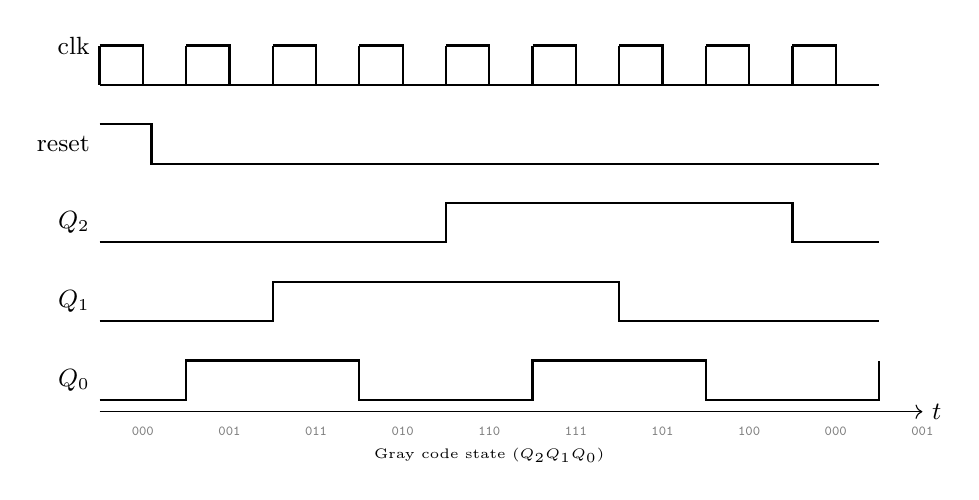
\begin{tikzpicture}[x=0.55cm, y=0.5cm]

  % ---- helper macro: draw a digital signal ----
  % Usage: \signal{label}{y}{list of (t,val) pairs with period 10}

  % Clock
  \node[anchor=east] at (0, 9) {\small clk};
  \foreach \t in {0,2,4,6,8,10,12,14,16} {
    \draw[thick] (\t,8) -- (\t,8) -- (\t,9);
    \draw[thick] (\t,9) -- (\t+1,9) -- (\t+1,8) -- (\t+2,8);
  }
  \draw[thick] (0,8) -- (18,8);

  % Reset: high 0-1.2, then low
  \node[anchor=east] at (0, 6.5) {\small reset};
  \draw[thick] (0,7) -- (1.2,7) -- (1.2,6) -- (18,6);

  % Q values after reset falls at t=1.2; first capture edge at t=2
  % t=2:  Q=001,  t=4:  Q=011,  t=6:  Q=010
  % t=8:  Q=110,  t=10: Q=111,  t=12: Q=101
  % t=14: Q=100,  t=16: Q=000,  t=18: Q=001 (repeat)

  % Draw Q2
  \node[anchor=east] at (0, 4.5) {\small $Q_2$};
  % 0..2: reset=0; 2..8: Q2=0; 8..16: Q2=1; 16..18: Q2=0
  \draw[thick] (0,4) -- (8,4) -- (8,5) -- (16,5) -- (16,4) -- (18,4);

  % Draw Q1
  \node[anchor=east] at (0, 2.5) {\small $Q_1$};
  % Q1 values per state: 000=0,001=0,011=1,010=1,110=1,111=1,101=0,100=0
  % edge at 2->0, 4->1, 8->1(no chg at 6), 12->0, 16->0(no chg)
  \draw[thick] (0,2) -- (4,2) -- (4,3) -- (12,3) -- (12,2) -- (18,2);

  % Draw Q0
  \node[anchor=east] at (0, 0.5) {\small $Q_0$};
  % Q0 values: 000=0,001=1,011=1,010=0,110=0,111=1,101=0... wait, let me redo
  % After reset, on edge at t=2: 000->001 => Q0 goes 0->1
  % t=4: 001->011, Q0 stays 1
  % t=6: 011->010, Q0 goes 1->0
  % t=8: 010->110, Q0 stays 0
  % t=10: 110->111, Q0 goes 0->1
  % t=12: 111->101, Q0 stays 1
  % t=14: 101->100, Q0 goes 1->0
  % t=16: 100->000, Q0 stays 0
  % t=18: 000->001, Q0 goes 0->1
  \draw[thick] (0,0) -- (2,0) -- (2,1) -- (6,1) -- (6,0) -- (10,0) -- (10,1) -- (14,1) -- (14,0) -- (18,0) -- (18,1);

  % State labels
  \foreach \t/\s in {0/000, 2/001, 4/011, 6/010, 8/110, 10/111, 12/101, 14/100, 16/000, 18/001} {
    \node[font=\tiny, gray] at (\t+1, -0.8) {\texttt{\s}};
  }
  \node[font=\tiny] at (9, -1.4) {Gray code state ($Q_2Q_1Q_0$)};

  % time axis
  \draw[->] (0,-0.3) -- (19,-0.3) node[right] {\small $t$};

\end{tikzpicture}
\caption{Simulated waveform for the 3-bit Gray code counter.  After reset, the output
$Q_2Q_1Q_0$ advances through the complete Gray code sequence (000, 001, 011, 010, 110,
111, 101, 100) on successive rising clock edges.  Only one bit changes at each
transition, confirming correct Gray code behavior.}
\end{figure}

% ─────────────────────────────────────────────
\subsection{State Transition Diagram and K-maps for $D_2$, $D_1$, $D_0$}

\subsubsection*{Next-State Table}

The 3-bit Gray code sequence defines the following next-state (and thus D-input) table:

\begin{center}
\begin{tabular}{|ccc|ccc|ccc|}
  \hline
  $Q_2$ & $Q_1$ & $Q_0$ & $Q_2^+$ & $Q_1^+$ & $Q_0^+$ & $D_2$ & $D_1$ & $D_0$ \\
  \hline
  0 & 0 & 0 & 0 & 0 & 1 & 0 & 0 & 1 \\
  0 & 0 & 1 & 0 & 1 & 1 & 0 & 1 & 1 \\
  0 & 1 & 1 & 0 & 1 & 0 & 0 & 1 & 0 \\
  0 & 1 & 0 & 1 & 1 & 0 & 1 & 1 & 0 \\
  1 & 1 & 0 & 1 & 1 & 1 & 1 & 1 & 1 \\
  1 & 1 & 1 & 1 & 0 & 1 & 1 & 0 & 1 \\
  1 & 0 & 1 & 1 & 0 & 0 & 1 & 0 & 0 \\
  1 & 0 & 0 & 0 & 0 & 0 & 0 & 0 & 0 \\
  \hline
\end{tabular}
\end{center}

\subsubsection*{State Transition Diagram}

\begin{figure}[H]
\centering
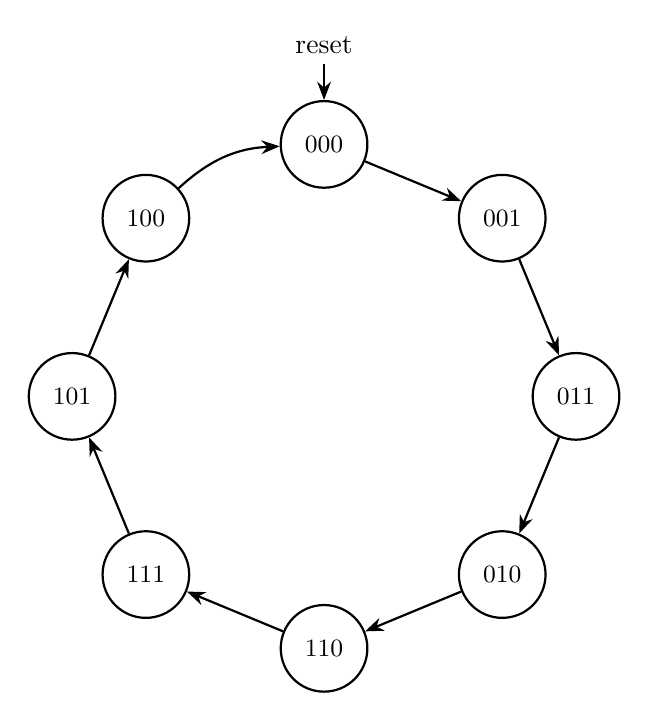
\begin{tikzpicture}[->, >=Stealth, thick,
    every state/.style={minimum size=1.1cm, font=\small}]

  % Place 8 states in a circle
  \node[state, initial, initial text=reset, initial where=above]
    (s0) at (90:3.2cm)  {000};
  \node[state]
    (s1) at (45:3.2cm)  {001};
  \node[state]
    (s2) at (0:3.2cm)   {011};
  \node[state]
    (s3) at (-45:3.2cm) {010};
  \node[state]
    (s4) at (-90:3.2cm) {110};
  \node[state]
    (s5) at (-135:3.2cm){111};
  \node[state]
    (s6) at (180:3.2cm) {101};
  \node[state]
    (s7) at (135:3.2cm) {100};

  \path (s0) edge (s1)
        (s1) edge (s2)
        (s2) edge (s3)
        (s3) edge (s4)
        (s4) edge (s5)
        (s5) edge (s6)
        (s6) edge (s7)
        (s7) edge [bend left=20] (s0);

\end{tikzpicture}
\caption{State transition diagram for the 3-bit Gray code counter. Each state is labeled
with its Gray code value $Q_2Q_1Q_0$. There are no external inputs; the counter advances
one state per rising clock edge and cycles back to 000 after 100.}
\end{figure}

\subsubsection*{Karnaugh Map for $D_2$}

\begin{center}
\begin{tabular}{|c|c|cccc|}
  \hline
  \multicolumn{2}{|c|}{$D_2$} & \multicolumn{4}{c|}{$Q_1 Q_0$} \\
  \multicolumn{2}{|c|}{}      & 00 & 01 & 11 & 10 \\
  \hline
  \multirow{2}{*}{$Q_2$} & 0  & 0  & 0  &  0 & \fbox{1} \\
                          & 1  & 0  & \fbox{1}  & \fbox{1} & \fbox{1} \\
  \hline
\end{tabular}
\end{center}

\begin{itemize}
  \item \textbf{Group 1 (2 cells):}
        $(Q_2{=}0,\,Q_1Q_0{=}10)$ and $(Q_2{=}1,\,Q_1Q_0{=}10)$:
        $Q_1=1$, $Q_0=0$ $\Rightarrow$ $Q_1\overline{Q_0}$.
  \item \textbf{Group 2 (2 cells):}
        $(Q_2{=}1,\,Q_1Q_0{=}01)$ and $(Q_2{=}1,\,Q_1Q_0{=}11)$:
        $Q_2=1$, $Q_0=1$ $\Rightarrow$ $Q_2 Q_0$.
\end{itemize}

\[
  \boxed{D_2 = Q_1\overline{Q_0} + Q_2 Q_0}
\]

\subsubsection*{Karnaugh Map for $D_1$}

\begin{center}
\begin{tabular}{|c|c|cccc|}
  \hline
  \multicolumn{2}{|c|}{$D_1$} & \multicolumn{4}{c|}{$Q_1 Q_0$} \\
  \multicolumn{2}{|c|}{}      & 00 & 01 & 11 & 10 \\
  \hline
  \multirow{2}{*}{$Q_2$} & 0  & 0  & \fbox{1} & \fbox{1} & \fbox{1} \\
                          & 1  & 0  & 0  &  0 & \fbox{1} \\
  \hline
\end{tabular}
\end{center}

\begin{itemize}
  \item \textbf{Group 1 (2 cells):}
        $(Q_2{=}0,\,Q_1Q_0{=}01)$ and $(Q_2{=}0,\,Q_1Q_0{=}11)$:
        $Q_2=0$, $Q_0=1$ $\Rightarrow$ $\overline{Q_2}\,Q_0$.
  \item \textbf{Group 2 (2 cells):}
        $(Q_2{=}0,\,Q_1Q_0{=}10)$ and $(Q_2{=}1,\,Q_1Q_0{=}10)$:
        $Q_1=1$, $Q_0=0$ $\Rightarrow$ $Q_1\overline{Q_0}$.
\end{itemize}

\[
  \boxed{D_1 = \overline{Q_2}\,Q_0 + Q_1\overline{Q_0}}
\]

Note that the term $Q_1\overline{Q_0}$ appears in both $D_2$ and $D_1$, so the
corresponding NAND gate is shared in the hardware implementation.

\subsubsection*{Karnaugh Map for $D_0$}

\begin{center}
\begin{tabular}{|c|c|cccc|}
  \hline
  \multicolumn{2}{|c|}{$D_0$} & \multicolumn{4}{c|}{$Q_1 Q_0$} \\
  \multicolumn{2}{|c|}{}      & 00 & 01 & 11 & 10 \\
  \hline
  \multirow{2}{*}{$Q_2$} & 0  & \fbox{1} & \fbox{1} & 0 & 0 \\
                          & 1  & 0  & 0  & \fbox{1} & \fbox{1} \\
  \hline
\end{tabular}
\end{center}

\begin{itemize}
  \item \textbf{Group 1 (2 cells):}
        $(Q_2{=}0,\,Q_1Q_0{=}00)$ and $(Q_2{=}0,\,Q_1Q_0{=}01)$:
        $Q_2=0$, $Q_1=0$ $\Rightarrow$ $\overline{Q_2}\,\overline{Q_1}$.
  \item \textbf{Group 2 (2 cells):}
        $(Q_2{=}1,\,Q_1Q_0{=}11)$ and $(Q_2{=}1,\,Q_1Q_0{=}10)$:
        $Q_2=1$, $Q_1=1$ $\Rightarrow$ $Q_2 Q_1$.
\end{itemize}

\[
  \boxed{D_0 = \overline{Q_2}\,\overline{Q_1} + Q_2 Q_1}
\]

This expression is equivalent to $\overline{Q_2 \oplus Q_1}$ (XNOR), meaning $D_0$ is 1
whenever $Q_2$ and $Q_1$ are equal.

\subsubsection*{AND-XOR-INV Implementation}

Observing that the product terms in $D_2$ and $D_1$ are mutually exclusive (they
cannot both be 1 at the same time), the OR can be replaced by XOR:

\begin{align*}
  D_2 &= (Q_1 \cdot \overline{Q_0}) \oplus (Q_2 \cdot Q_0) \\
  D_1 &= (\overline{Q_2} \cdot Q_0) \oplus (Q_1 \cdot \overline{Q_0}) \\
  D_0 &= \overline{Q_2 \oplus Q_1}
\end{align*}

This maps directly onto the available ICs:
\begin{itemize}
  \item \textbf{SN74LS08N (AND):} compute $Q_1\cdot\overline{Q_0}$ (shared between
        $D_2$ and $D_1$), $Q_2\cdot Q_0$, and $\overline{Q_2}\cdot Q_0$
        --- 3 of 4 gates used.
  \item \textbf{SN74LS86AN (XOR):} compute $D_2$, $D_1$, and $Q_2 \oplus Q_1$
        --- 3 of 4 gates used.
  \item \textbf{SN74LS04N (INV):} invert $Q_2 \oplus Q_1$ to produce $D_0$
        --- 1 of 6 inverters used.
\end{itemize}

All complemented state signals ($\overline{Q_0}$, $\overline{Q_1}$, $\overline{Q_2}$)
are taken directly from the $\overline{Q}$ outputs of the SN74LS109AN flip-flops,
requiring no additional inverters for those signals.  The term $Q_1\cdot\overline{Q_0}$
is shared between $D_2$ and $D_1$, reducing the AND gate count to three.

% ─────────────────────────────────────────────
\subsection{Wiring Diagrams}

\subsubsection*{Original Circuit -- Gray Code Counter with LED Output}

The circuit uses two SN74LS109AN ICs (three of the four JK flip-flops are used for
$Q_2$, $Q_1$, $Q_0$), one SN74LS08N (AND), one SN74LS86AN (XOR), and one SN74LS04N
(inverter).  Each flip-flop is configured as a DFF by connecting both $J$ and
$\overline{K}$ to the same $D$ input signal.  The key wiring connections are:

\begin{center}
\small
\begin{tabular}{ll}
  \toprule
  \textbf{Signal} & \textbf{Connection} \\
  \midrule
  CLK (all 3 FFs)              & Function generator 1\,Hz CMOS output \\
  $\overline{\text{CLR}}$ (all 3 FFs) & Reset button (active-low; pull-up resistor to $V_{DD}$) \\
  $\overline{\text{PRE}}$ (all 3 FFs) & $V_{DD}$ (preset disabled) \\
  $J_2 = \overline{K}_2 = D_2$ & XOR output: $(Q_1\cdot\overline{Q_0}) \oplus (Q_2\cdot Q_0)$ \\
  $J_1 = \overline{K}_1 = D_1$ & XOR output: $(\overline{Q_2}\cdot Q_0) \oplus (Q_1\cdot\overline{Q_0})$ \\
  $J_0 = \overline{K}_0 = D_0$ & INV output: $\overline{Q_2 \oplus Q_1}$ \\
  $\overline{Q_0},\overline{Q_1},\overline{Q_2}$ & Taken from $\overline{Q}$ pins of SN74LS109AN (no extra inverter) \\
  $Q_2,\,Q_1,\,Q_0$            & LED anodes (through 330\,$\Omega$ resistors to GND) \\
  \bottomrule
\end{tabular}
\end{center}

\begin{figure}[H]
\centering
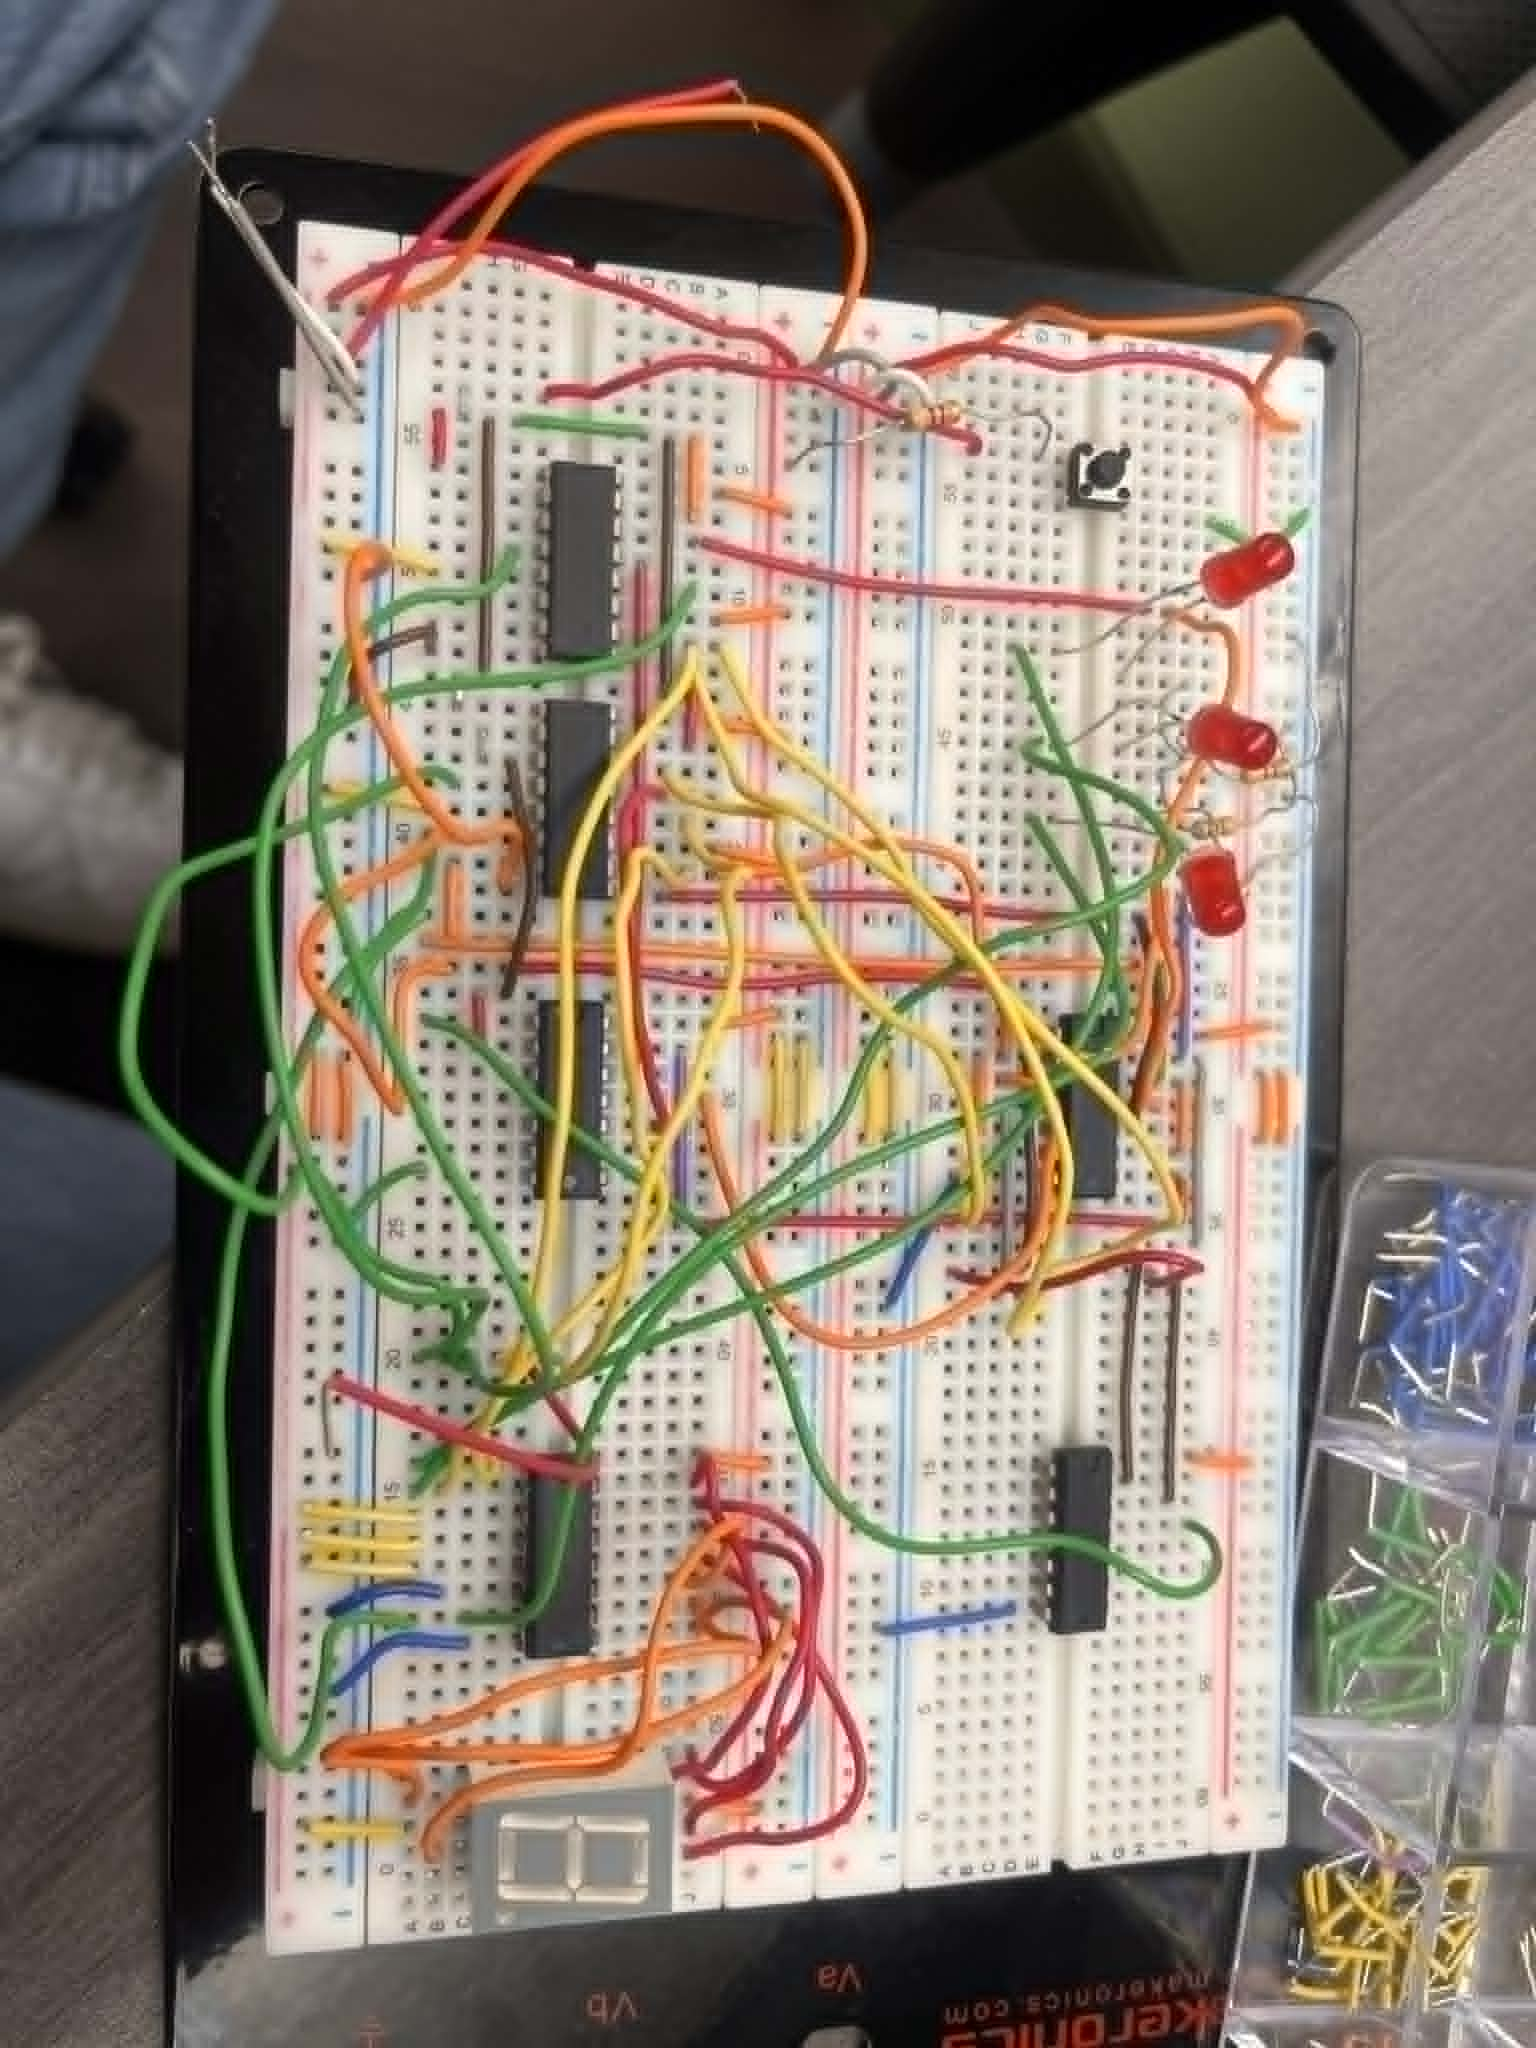
\includegraphics[width=0.72\linewidth]{cda_lab7-circuit.jpg}
\caption{Breadboard implementation of the 3-bit Gray code counter.  The two 74LS74 DFF
ICs (center) provide the three flip-flops and their complemented outputs.  The 74LS00
NAND IC (lower center) implements the minimized next-state logic.  The three red LEDs
(right) display the current Gray code value $Q_2Q_1Q_0$.  A push button (top) is wired
with a pull-up resistor to the active-low CLR pins for reset.}
\end{figure}

\begin{center}
  \small\textbf{Supplementary Video:}
  \href{https://drive.google.com/file/d/1hqkrgtYiLh8mPWMN8gT19IOGA3trhYUO/view?usp=sharing}{Circuit Demonstration Recording (Google Drive)}
\end{center}

\subsubsection*{Modified Circuit -- Gray Code Counter with 7-Segment Display}

In the modified circuit the three LEDs are replaced by the 74LS47N BCD-to-7-segment
decoder/driver and a common-anode 7-segment display.  The counter outputs $Q_2$, $Q_1$,
$Q_0$ are connected to inputs $C$, $B$, $A$ of the 74LS47N respectively (MSB to LSB).
All 74LS47N segment outputs ($\overline{a}$–$\overline{g}$, active-low) drive the
corresponding segments of the display through current-limiting resistors (330\,$\Omega$
recommended to avoid exceeding the display's forward current rating).  The $\overline{\text{LT}}$,
$\overline{\text{RBI}}$, and $\overline{\text{BI/RBO}}$ inputs on the 74LS47N are tied to
$V_{DD}$ to keep lamp-test and blanking inactive.  The rest of the counter circuit
(DFFs, NAND logic, clock, reset) remains unchanged.

\begin{center}
\small
\begin{tabular}{ll}
  \toprule
  \textbf{74LS47N Pin} & \textbf{Connection} \\
  \midrule
  $A$ (pin 7)          & Counter $Q_0$ \\
  $B$ (pin 1)          & Counter $Q_1$ \\
  $C$ (pin 2)          & Counter $Q_2$ \\
  $D$ (pin 6)          & GND (no 4th bit) \\
  $\overline{\text{LT}}$ (pin 3)  & $V_{DD}$ \\
  $\overline{\text{RBI}}$ (pin 5) & $V_{DD}$ \\
  $\overline{\text{BI/RBO}}$ (pin 4) & $V_{DD}$ \\
  Segment outputs $\overline{a}$--$\overline{g}$ (pins 9--15) & 7-segment display segments a--g via 330\,$\Omega$ \\
  Common anode (display) & $V_{DD}$ \\
  $V_{CC}$ (pin 16)    & 5\,V \\
  GND (pin 8)          & GND \\
  \bottomrule
\end{tabular}
\end{center}

% ─────────────────────────────────────────────
\section{Discussion}

The circuit behaved as expected.  After asserting reset, all three LEDs were off
($Q_2Q_1Q_0 = 000$).  With the function generator providing a 1\,Hz clock, the LEDs
cycled through the Gray code sequence at a rate slow enough to observe each state change
visually.  Crucially, only one LED changed state at each clock edge, confirming the
single-bit-change property of Gray code and validating our next-state logic.

The K-map simplification produced compact excitation equations.  Because the two
product terms in $D_2$ and $D_1$ are mutually exclusive, OR can be replaced by XOR,
enabling a clean implementation with SN74LS08N AND gates and SN74LS86AN XOR gates.
The term $Q_1\cdot\overline{Q_0}$ is shared between $D_2$ and $D_1$, reducing the AND
gate count to three (within a single SN74LS08N IC).  The SN74LS109AN JK flip-flop,
configured as a DFF by connecting $J = \overline{K} = D$, provided both $Q$ and
$\overline{Q}$ outputs natively, supplying all complemented state signals without
requiring additional inverter gates.  The SN74LS04N was used solely to invert the XOR
output for $D_0 = \overline{Q_2 \oplus Q_1}$.

The expression $D_0 = \overline{Q_2 \oplus Q_1}$ has an intuitive interpretation: the
LSB of the next Gray code state is 1 whenever the two MSBs of the current state are
equal, and 0 otherwise.  This reflects the mirror symmetry of the Gray code sequence
across its midpoint.

In the 7-segment display extension, the display shows digit values 0--7 in the order 0,
1, 3, 2, 6, 7, 5, 4 (the decimal equivalents of the Gray code words), which is visually
non-monotonic but demonstrates the counter's correct Gray-code sequencing.

% ─────────────────────────────────────────────
\section{Conclusion}

In this lab we designed and implemented a 3-bit Gray code up counter.  We derived the
next-state table, simplified the excitation equations for $D_2$, $D_1$, and $D_0$
using Karnaugh maps, and implemented the logic using SN74LS08N AND gates and SN74LS86AN
XOR gates, with a single SN74LS04N inverter for $D_0$.  The SN74LS109AN JK flip-flops,
configured as DFFs via $J = \overline{K} = D$, served as the memory elements and
provided $\overline{Q}$ outputs that eliminated the need for extra inverters.  A Verilog
behavioral model and testbench confirmed the expected waveform.  The breadboard circuit,
clocked at 1\,Hz, successfully cycled through all eight Gray code states with exactly
one LED changing per clock edge.  The optional extension connected the counter to a
SN74LS47N and 7-segment display, further demonstrating the circuit's correct operation.

\end{document}
